\section{Introducción}
En esta segunda etapa del proyecto de diseño, construcción y puesta en servicio de la nueva subestación Huila 230 kV y sus líneas de transmisión asociadas, se abordan con mayor profundidad los criterios técnicos de diseño exigidos en la convocatoria pública. Este avance se enfoca en el análisis detallado de las especificaciones contenidas en el Anexo 1 de la convocatoria de la UPME, complementadas con los lineamientos establecidos en el Código de Redes (Resolución CREG 025 de 1995 y CREG 098 de 2000), el Reglamento Técnico de Instalaciones Eléctricas (RETIE) y las disposiciones ambientales aplicables.\\ Se revisaron parámetros clave como la potencia nominal en el lado receptor, la capacidad de corriente del circuito, la resistencia DC por fase, los niveles máximos de radio-interferencia y ruido audible, la regulación de tensión, el límite térmico, el tipo de conductor permitido y las condiciones para evitar el efecto corona. Adicionalmente, se evaluaron distintas configuraciones de diseño eléctrico que incluyeron opciones de circuito sencillo y doble circuito con conductores en haz, dispuestos horizontalmente o en triángulo, con separación de 45,72 cm. Se compararon también diferentes tipos de torre y combinaciones de conductores, a fin de asegurar la viabilidad técnica y económica de la solución seleccionada. La configuración final fue escogida con base en su cumplimiento con los parámetros normativos y su conveniencia desde el punto de vista operativo y económico. Finalmente, se calcularon y organizaron en tablas las condiciones eléctricas de operación en ambos extremos de la línea (emisor y receptor), incluyendo datos relevantes como el SIL, la potencia natural, la regulación de tensión, las pérdidas de potencia y demás variables que respaldan la selección técnica.\\ En base a los lineamientos técnicos es posible asegurar que las soluciones propuestas cumplan con los estándares de cálidad, seguridad y eficiencia exigidos para garantizar una operación confiable del sistema. \\Además, se presenta el análisis del trazado propuesto de la línea, identificando la ruta óptima mediante herramientas geográficas como Google Earth, y considerando criterios técnicos, ambientales y topográficos. 




\section{PARÁMETROS DE DISEÑO Y SELECCIÓN DE LA RUTA}

Para la contrucción de la línea de transmisión Huila 230 kV se tomaron en cuenta espeficicaciones y criterios técnicos de diseño basados en el RETIE, CREG y la UPME. Contemplando una potencia nóminal de 700 MVA y un factor de potencia de 0.9 en atraso, se cálcula la corriente en el lado receptor que da un valor de 1757 [A]. Para la elección de conductor es muy importante analizar la capacidad de corriente de operación del circuito para evitar que el conductor se sobrecaliente o se dañe, en este caso, se toma una mayor a 2400 amperios a temperatura ambiente máxima promedio y se toma resistencia DC a 20 grados Celsius como 0,0230 ohmios/km.\\
Uno de los efectos de gran importancia en líneas de transmisión (LT) es el efecto corona, este es un fenómeno eléctrico causado por la ionización del aire circundante a los conductores eléctricos debido a la colisión de electrones libres que se escapan del sistema. En el momento que las moléculas de aire se ionizan, éstas son capaces de conducir la corriente eléctrica y parte de los electrones que circulan por la línea pasan a circular por el aire. Cuando ocurre el Efecto Corona este crea ozono, el ozono deteriora material dieléctrico con base de goma y/o plástico; si existen condiciones de humedad el ozono puede crear ácido nítrico que es capaz de atacar al cobre y otros metales causando corrosión, por tanto en la construcción de la línea no se deberá presentar efecto corona en condiciones de buen tiempo; y es a raíz de este que se desarrollan fenómenos tales como la radio interferencia (degradación de una señal de radio que perturba la recepción de radio, televisión, teléfonos inalámbricos y otros dispositivos) y el ruido audible (zumbido), los cuales con el aumento de la tensión de operación se hacen cada vez más notorios, y aumentan así la posibilidad de que tanto personas como equipos puedan ser afectados o interferidos debido a las propiedades electromagnéticas que se generan en los alrededores de la LT. Por eso todos los equipos y conectores deberán ser contruidos cumpliendo a una relación señal-ruido mínima de: a) Zona Rurales: 22 dB a 80m del eje de la línea a 1000 kHz en condiciones de buen tiempo y b) Zonas Urbanas: 22 dB a 40m del eje de la línea a 1000 kHz en condiciones de buen tiempo y en cuanto a ruido audible generado por la línea y/o la subestación, deberá limitarse a los estándares máximos permisibles de niveles de emisión de ruido establecidos en Resolución 0627 de 2006 (abril 7) Ministerio de Ambiente y Desarrollo Sostenible.\\
Para la correcta elección del conductor, también se consideró el cumplimiento de la regulación de tensión, que debe estar dentro del rango permitido de ±10 \%. Además, se verificó el límite térmico, asegurando que la temperatura del conductor bajo condiciones normales de operación no supere los 75 °C. Las pérdidas por efecto Joule también se controlaron, garantizando que no excedan el 3 \% por cada 100 km de línea, tomando como base la resistencia del conductor a 75 °C.\\
Como parte del diseño del sistema de transmisión a 230 kV en el departamento del Huila, se planteó inicialmente una interconexión eléctrica entre tres subestaciones: Subestación Betania, Nueva Subestación Huila y Subestación Tuluní. Para ello, se realizó una evaluación general del territorio utilizando la herramienta Google Earth Pro, lo cual permitió identificar un trazado preliminar que conecta las tres subestaciones, evaluando condiciones topográficas, uso del suelo, áreas sensibles, cuerpos de agua y cercanía a centros poblados.\\
La ruta general del proyecto tiene una longitud aproximada de 160,45 km, atravesando principalmente zonas rurales, con tramos de topografía montañosa y presencia agrícola. Esta visión integral sirvió como base para la planeación técnica y estratégica del sistema de transmisión.\\

\begin{figure}[!ht]
\centering
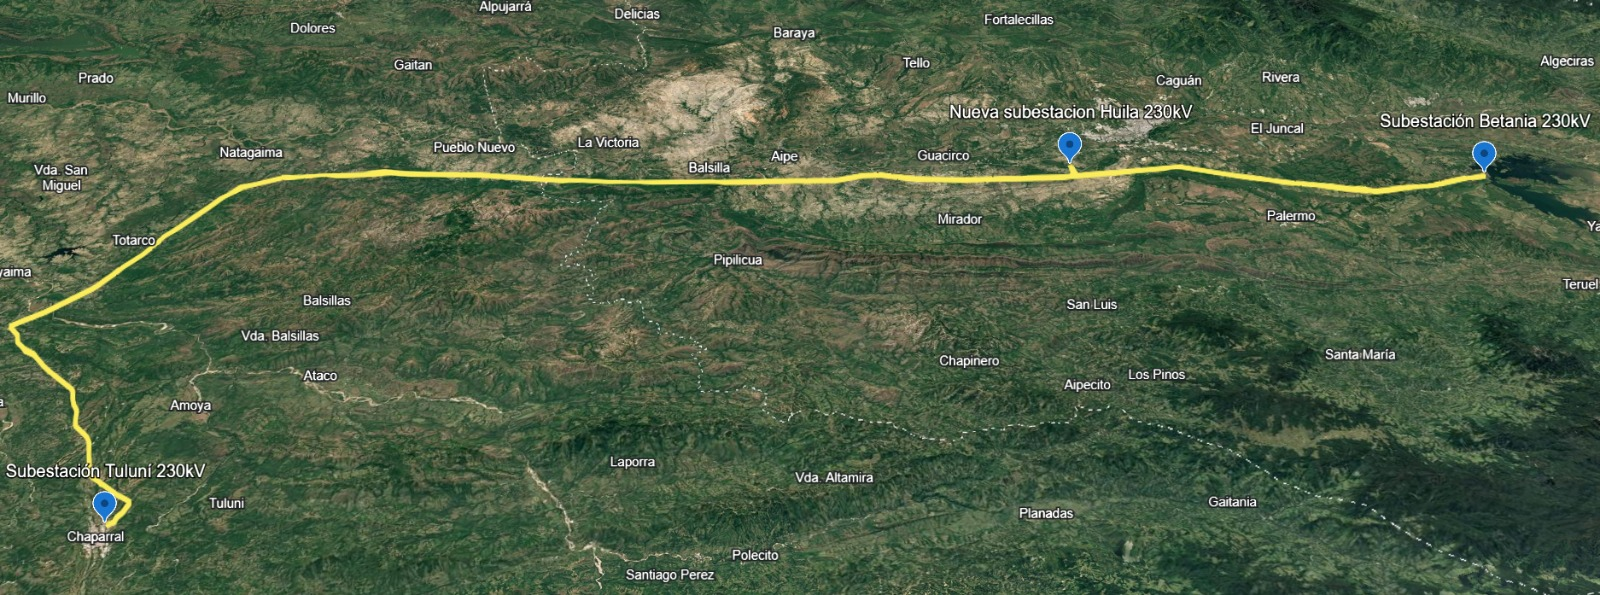
\includegraphics[width=1\linewidth]{img/Trazado.jpg}
\caption{Trazado general del sistema con Google Earth.}
\label{fig:general}
\end{figure}
Si bien el proyecto contempla un sistema de mayor longitud, el análisis técnico y eléctrico detallado se centró exclusivamente en el tramo comprendido entre la Subestación Betania y la Nueva Subestación Huila, con una longitud aproximada de 31 km. Este segmento fue seleccionado por presentar condiciones topográficas representativas del recorrido general, y por su relevancia estratégica en la primera fase del proyecto.

Para este tramo se realizó un trazado más preciso utilizando también Google Earth Pro, lo cual permitió identificar una ruta técnicamente viable que evita interferencias con zonas urbanas o áreas de protección ambiental. El entorno geográfico cercano a la nueva subestación Huila fue evaluado en detalle, considerando aspectos como accesibilidad, pendientes y cercanía a corredores de infraestructura existentes. Este tramo fue tomado como referencia para el cálculo de parámetros eléctricos, estudios de diseño geométrico y evaluación de fenómenos como el efecto corona, dada su representatividad y factibilidad técnica dentro del sistema propuesto.

\begin{figure}[!ht]
\centering
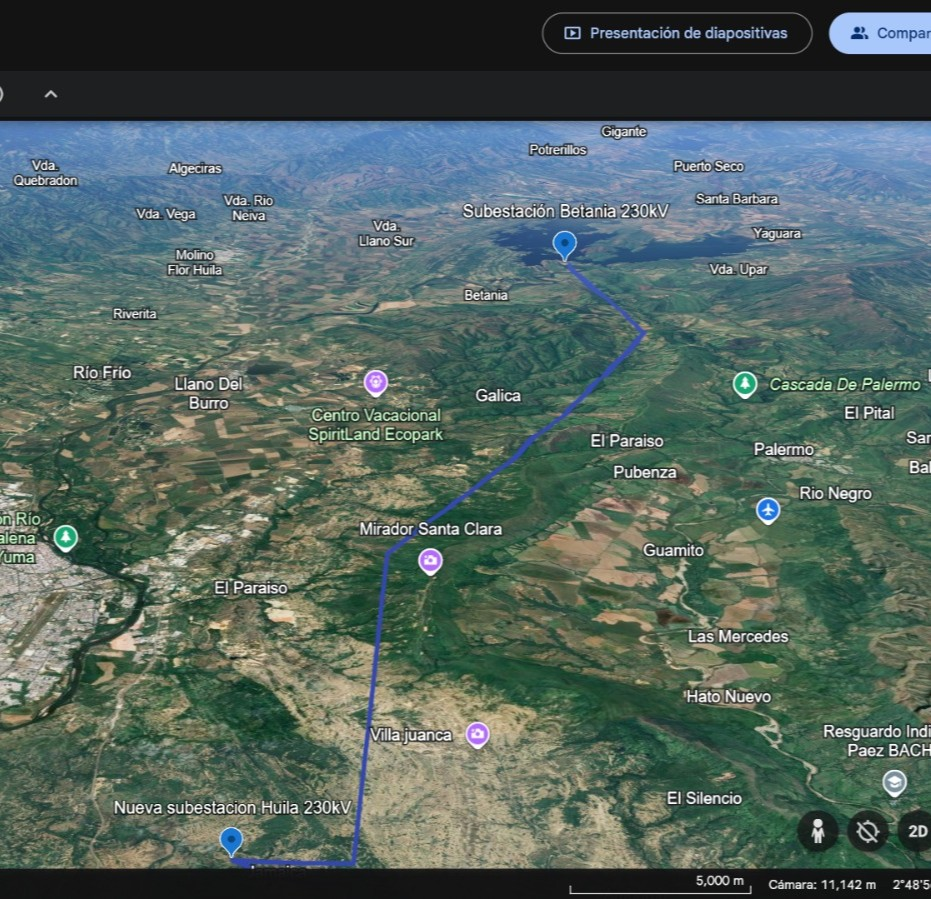
\includegraphics[width=0.48\linewidth]{img/conexion.jpg}
\caption{Trazado Línea Betania - Huila.}
\label{fig:tramoBH}
\end{figure}

Este tramo fue tomado como referencia para el cálculo de parámetros eléctricos, estudios de diseño geométrico, modelado de cargas, y evaluación de fenómenos como el efecto corona, dada su representatividad y factibilidad técnica dentro del sistema propuesto.

\section*{Criterios de selección del trazado y evaluación de alternativas}

Para la selección del trazado se evaluaron distintos criterios técnicos, geográficos y ambientales que permitieran definir el recorrido más adecuado. A continuación, se resumen los aspectos más relevantes:

\begin{itemize}
    \item Se priorizó el paso por zonas con pendientes moderadas y buena accesibilidad, lo que facilita tanto la construcción como el mantenimiento futuro de la línea.
    
    \item Se evitó que el trazado atravesara áreas urbanas, centros poblados o zonas densamente habitadas, con el fin de reducir afectaciones sociales y costos asociados a servidumbres.
    
    \item Se buscó mantener una distancia prudente con áreas protegidas, zonas de valor ambiental o ecosistemas frágiles (como ríos y quebradas), para minimizar afectaciones y garantizar la estabilidad de las estructuras.
    
    \item Se procuró mantener el trazado cercano a vías ya existentes, lo cual facilita el transporte de materiales y el acceso para la construcción de torres.
    
    \item En cuanto a las alternativas de trazado, se evaluaron varias rutas con diferentes configuraciones y longitudes. Algunas opciones implicaban atravesar terrenos montañosos o con vegetación densa, lo que incrementaba la complejidad técnica y los costos de construcción. Otras alternativas ofrecían trayectos más accesibles, pero con mayor longitud total, lo que incrementaba las pérdidas eléctricas y los costos de operación.
\end{itemize}


Finalmente, la ruta seleccionada fue aquella que representó un equilibrio entre viabilidad técnica, facilidad de acceso, menor afectación ambiental y cercanía a infraestructuras existentes, como vías y caminos rurales. Esta decisión se apoyó tanto en el análisis geoespacial como en criterios de diseño 
eléctrico, buscando garantizar la confiabilidad del sistema y el cumplimiento de la normativa vigente.